\section{Introduction}
Motion parameter information is a necessary component in numerous applications. 
From robotic navigation, and collision detection to sport performance analysis, knowing an object's velocity is frequently needed \cite{kasiri2015combat,kasiri2017fine,wattanamongkhol2005method}. 
As more of these applications arise, the need grows for a computer vision based method to provide the appropriate motion parameter estimations \cite{marcon2010structural,miarka2011objectivity,polak2016motion}. 
Currently most motion parameter information has to be documented from devices on-board the moving object, such as IMUs (Inertial Measurement Unit) or via radars that are usually positioned knowing the object's path beforehand. 
In order to create a more useful and robust method to estimate motion parameters computer vision models are the logical next step.

\begin{figure}[t!]
    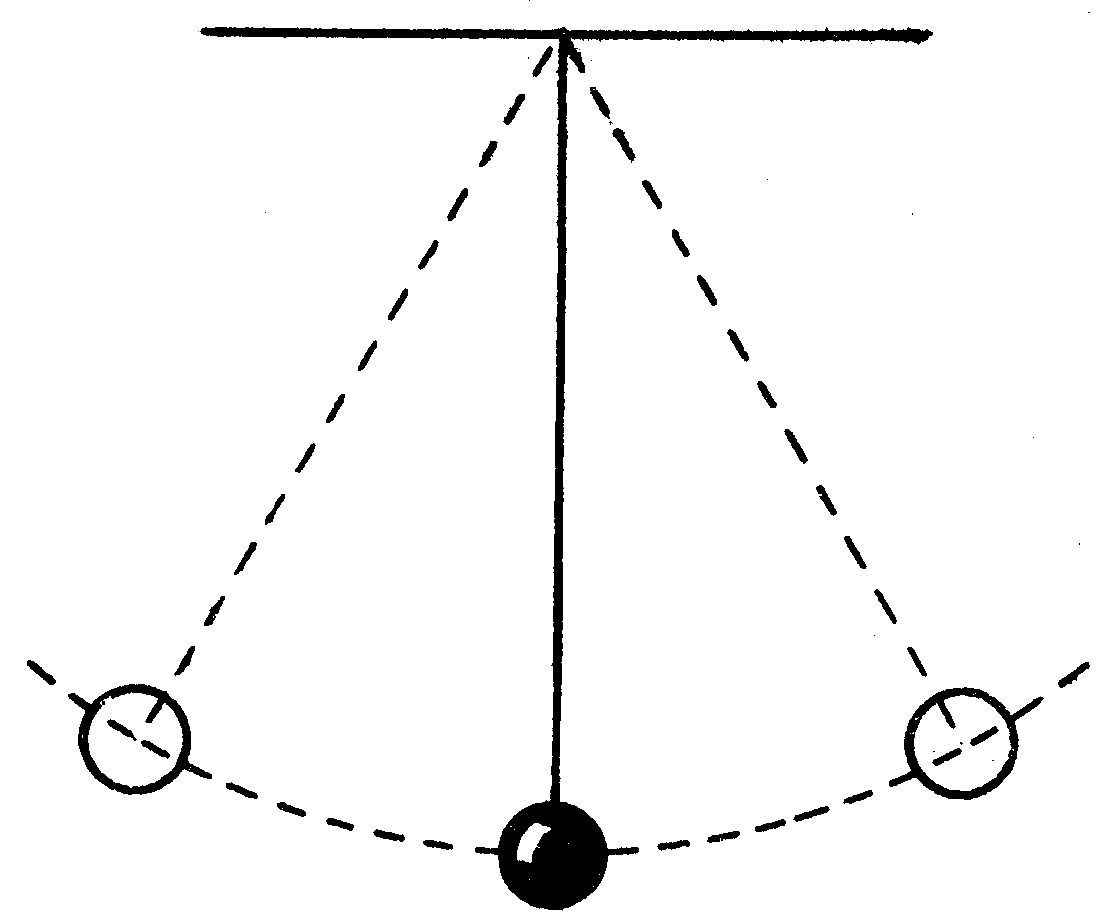
\includegraphics[width=1.0\columnwidth]{Images/pend.png}
    \caption{
    An example of the pendulum scene in the I-MOVE dataset.
    }\label{fig:pend.png} 
\end{figure}

In this paper, we introduce a new public RGB-D dataset to help address the above issues. 
The dataset features various outdoor and indoor scenes as opposed to most other RGB-D datasets which are frequently focused on static indoor environments. 
Our dataset also focuses on and provides annotations for a single moving object in each scene to best accommodate the greatest number of applications. 
The objects also vary though-out the scenes, for example some scenes are based upon a person's or dog's movements while others may be a rolling ball or pendulum as can be seen in Figure~\ref{fig:pend.png}. 


The main contribution of this dataset will be that each object's velocity will be provided in the ground truth. 
This allows people to train, test, and compare with the data. 
Taking another step to help bring the computer vision community closer to achieving accurate motion parameter estimation. 
The dataset includes training and test images that were captured from six different RGB-D camera views all time synchronized and with additional equipment (radar, motion capture, etc.) to verify calculated velocity and position ground truth. 
The camera type / model is also provided within the dataset. 
The cameras include: Three stereo setups of GoPro Hero 3s (six GoPros total), an Intel RealSense 435, Intel RealSense 415, and a ZED. 
This variety in devices helps to ensure the motion parameter estimation models will be as effective in the real world as possible.


\section{Motivation and Prior Works}
Vision-based velocity (or motion) estimation has been studied for decades. 
In recent years, as adequate cameras and computational power has become more accessible, the number of works attempting to estimate motion parameters has grown dramatically. 
Many of these works differ in the object and purpose for estimating motion parameters but all require a dataset with adequate ground truth and associate images.

From collision detection to athletic performance analysis, motion parameters are a crucial component to accuracy in these application. 
For example, to have an effective collision detection / time estimation model it is not only necessary to take into account your directional velocity but that of other objects. 
In order to accomplish this it is required that you have the three dimensional directional velocity of each of the objects within a reasonable view and distance.
Similarly, for object catching or throwing in the robotics field this information is essential to accurately estimating the trajectory / path of the object. 
For athlete performance analysis, numerous sports rely on velocity and acceleration information. 
Most obviously, sports where speed is the main component (running, biking, swimming, etc.), but also for sports such as weightlifting where the athletes are looking for their lift force and acceleration is required to calculate this, or for skateboarders attempting to add quantitative information to their training approach.

Prior attempts to estimate speed information in a relevant and accurate way have frequently relied on RGB-D data HERE


, where as those that used strictly RGB HERE


proved unreliable and too inaccurate to be plausible for real world applications. Due to the limited accuracy and possibility of successful estimations with purely RGB data or the existing RGB-D dataset, we found it necessary to create the I-MOVE dataset.
